\documentclass[tikz]{standalone}

\usetikzlibrary{arrows.meta}
\usetikzlibrary{positioning}
\usetikzlibrary{external}

\begin{document}
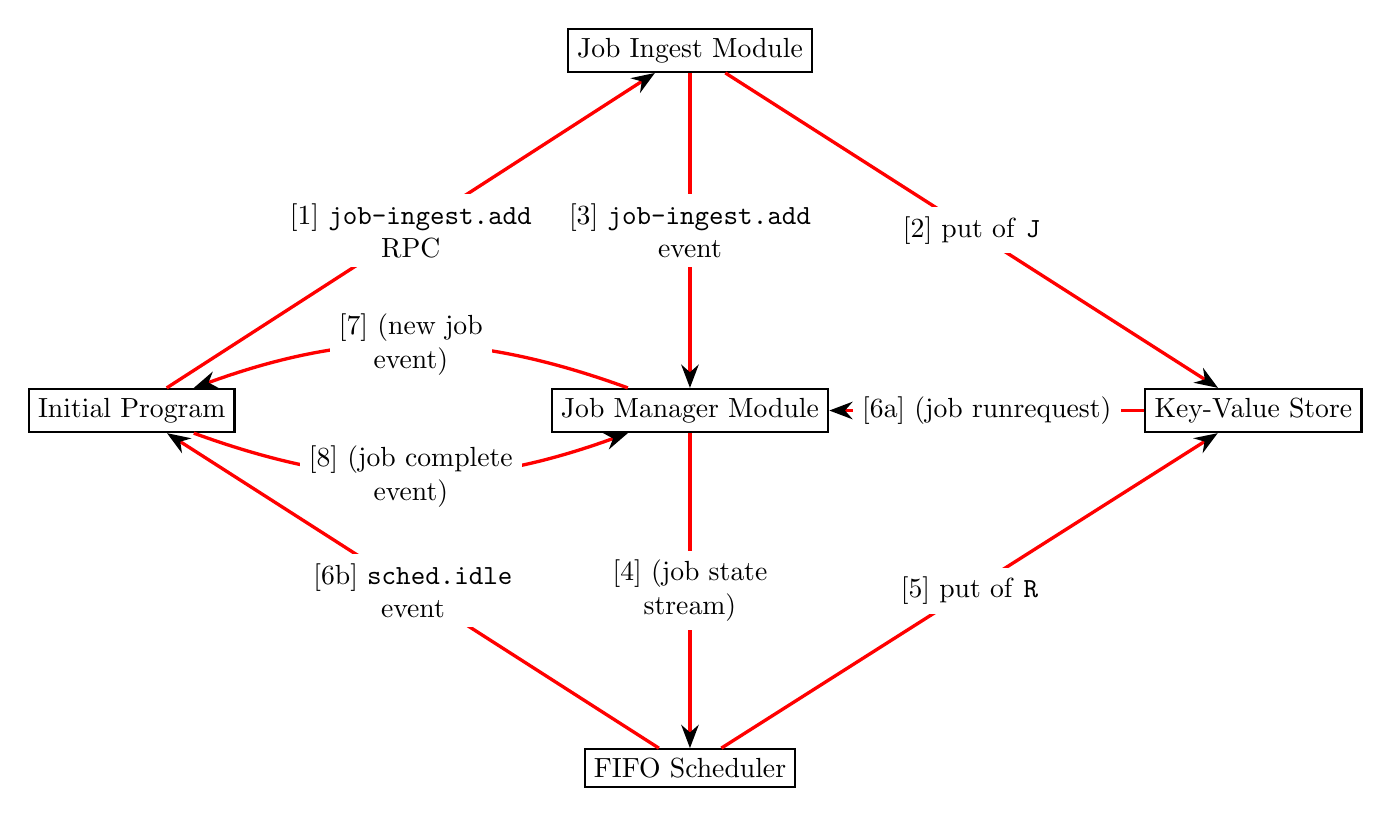
\begin{tikzpicture}
\begin{scope}[every node/.style={thick,draw,rectangle}]
    \node (init_prog) at (0,0)               {Initial Program};
    \node[right=4 of {init_prog}]     (job_man) {Job Manager Module};
    \node[above=4 of {job_man}]  (ingest)  {Job Ingest Module};
    \node[below=4 of {job_man}]    (sched)   {FIFO Scheduler};
    \node[right=4 of {job_man}]    (kvs)     {Key-Value Store};
\end{scope}

\newcounter{MajorEventCount}
\newcounter{MinorEventCount}
\setcounter{MajorEventCount}{1}
\newcommand{\newEvent}{\arabic{MajorEventCount}\stepcounter{MajorEventCount}\setcounter{MinorEventCount}{1}}
\setcounter{MinorEventCount}{1}
\newcommand{\newMinorEvent}{\arabic{MajorEventCount}\alph{MinorEventCount}\stepcounter{MinorEventCount}}

\begin{scope}[>={Stealth[black]},
              every node/.style={fill=white},
              every edge/.style={draw=red,very thick,align=center}]
    \path [->] (init_prog) edge                node {[\newEvent] \texttt{job-ingest.add} \\ RPC}  (ingest);
    \path [->] (ingest)    edge                node {[\newEvent] put of \texttt{J}} (kvs);
    \path [->] (ingest)    edge                node {[\newEvent] \texttt{job-ingest.add} \\ event} (job_man);
    \path [->] (job_man)   edge                node {[\newEvent] (job state \\ stream)} (sched);
    \path [->] (sched)     edge                node {[\newEvent] put of \texttt{R}} (kvs);
    \path [->] (kvs)       edge                node {[\newMinorEvent] (job runrequest)} (job_man);
    \path [->] (sched)     edge                node {[\newMinorEvent] \texttt{sched.idle} \\ event} (init_prog);
    \stepcounter{MajorEventCount}
    \path [->] (job_man)   edge[bend right=20] node {[\newEvent] (new job \\ event)} (init_prog);
    \path [->] (init_prog) edge[bend right=20] node {[\newEvent] (job complete \\ event)}  (job_man);
\end{scope}
\end{tikzpicture}
\end{document}

%%% Local Variables:
%%% mode: latex
%%% TeX-master: t
%%% End:
